% Graphic for TeX using PGF
% Title: /home/tomgli/workspace/github.com/bachopp/thesis/files/chapters/design/graphs/serverwebsocket.dia
% Creator: Dia v0.97.3
% CreationDate: Sat Apr 23 14:55:21 2016
% For: tomgli
% \usepackage{tikz}
% The following commands are not supported in PSTricks at present
% We define them conditionally, so when they are implemented,
% this pgf file will use them.
\ifx\du\undefined
  \newlength{\du}
\fi
\setlength{\du}{15\unitlength}
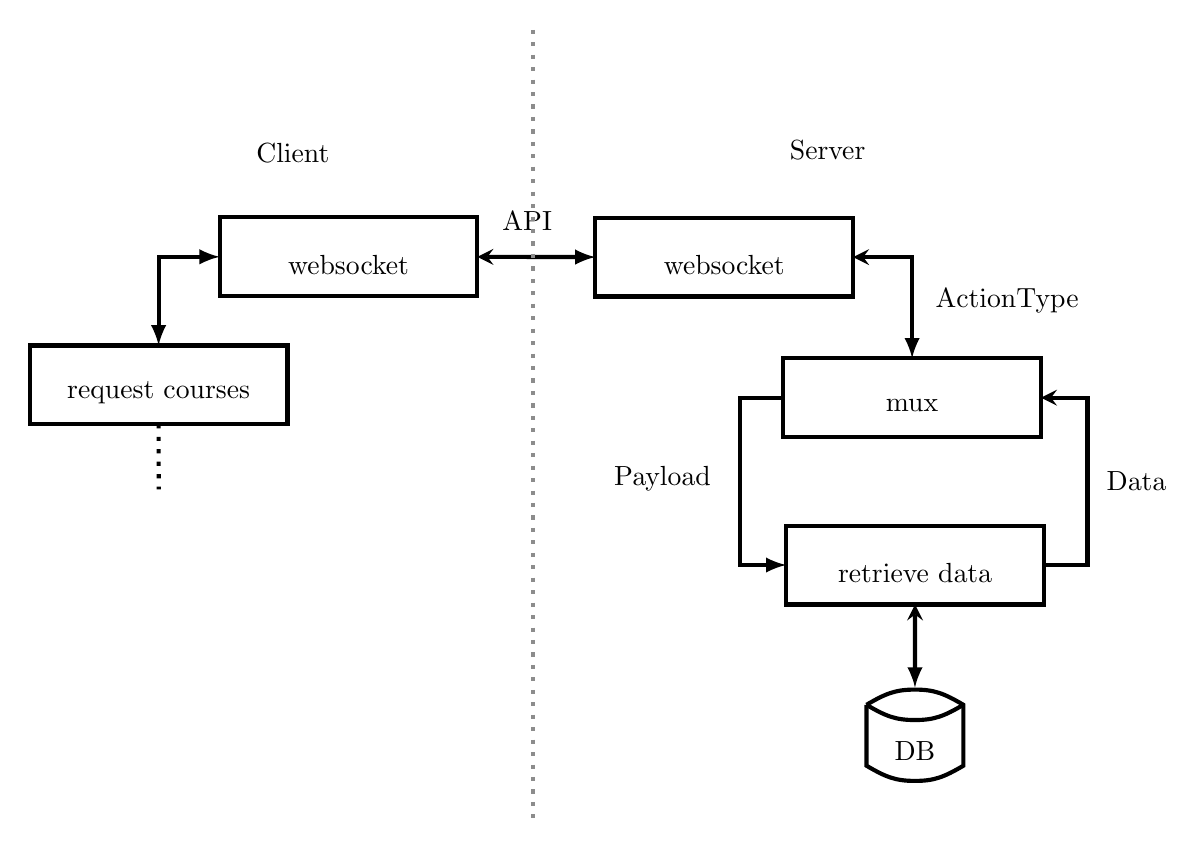
\begin{tikzpicture}
\pgftransformxscale{1.000000}
\pgftransformyscale{-1.000000}
\definecolor{dialinecolor}{rgb}{0.000000, 0.000000, 0.000000}
\pgfsetstrokecolor{dialinecolor}
\definecolor{dialinecolor}{rgb}{1.000000, 1.000000, 1.000000}
\pgfsetfillcolor{dialinecolor}
\definecolor{dialinecolor}{rgb}{1.000000, 1.000000, 1.000000}
\pgfsetfillcolor{dialinecolor}
\fill (16.302398\du,9.285788\du)--(16.302398\du,11.185788\du)--(22.509898\du,11.185788\du)--(22.509898\du,9.285788\du)--cycle;
\pgfsetlinewidth{0.100000\du}
\pgfsetdash{}{0pt}
\pgfsetdash{}{0pt}
\pgfsetmiterjoin
\definecolor{dialinecolor}{rgb}{0.000000, 0.000000, 0.000000}
\pgfsetstrokecolor{dialinecolor}
\draw (16.302398\du,9.285788\du)--(16.302398\du,11.185788\du)--(22.509898\du,11.185788\du)--(22.509898\du,9.285788\du)--cycle;
% setfont left to latex
\definecolor{dialinecolor}{rgb}{0.000000, 0.000000, 0.000000}
\pgfsetstrokecolor{dialinecolor}
\node at (19.406148\du,10.435788\du){request courses};
\definecolor{dialinecolor}{rgb}{1.000000, 1.000000, 1.000000}
\pgfsetfillcolor{dialinecolor}
\fill (20.877987\du,6.200760\du)--(20.877987\du,8.100760\du)--(27.085487\du,8.100760\du)--(27.085487\du,6.200760\du)--cycle;
\pgfsetlinewidth{0.100000\du}
\pgfsetdash{}{0pt}
\pgfsetdash{}{0pt}
\pgfsetmiterjoin
\definecolor{dialinecolor}{rgb}{0.000000, 0.000000, 0.000000}
\pgfsetstrokecolor{dialinecolor}
\draw (20.877987\du,6.200760\du)--(20.877987\du,8.100760\du)--(27.085487\du,8.100760\du)--(27.085487\du,6.200760\du)--cycle;
% setfont left to latex
\definecolor{dialinecolor}{rgb}{0.000000, 0.000000, 0.000000}
\pgfsetstrokecolor{dialinecolor}
\node at (23.981737\du,7.350760\du){websocket};
\definecolor{dialinecolor}{rgb}{1.000000, 1.000000, 1.000000}
\pgfsetfillcolor{dialinecolor}
\fill (29.928944\du,6.207449\du)--(29.928944\du,8.107449\du)--(36.136444\du,8.107449\du)--(36.136444\du,6.207449\du)--cycle;
\pgfsetlinewidth{0.100000\du}
\pgfsetdash{}{0pt}
\pgfsetdash{}{0pt}
\pgfsetmiterjoin
\definecolor{dialinecolor}{rgb}{0.000000, 0.000000, 0.000000}
\pgfsetstrokecolor{dialinecolor}
\draw (29.928944\du,6.207449\du)--(29.928944\du,8.107449\du)--(36.136444\du,8.107449\du)--(36.136444\du,6.207449\du)--cycle;
% setfont left to latex
\definecolor{dialinecolor}{rgb}{0.000000, 0.000000, 0.000000}
\pgfsetstrokecolor{dialinecolor}
\node at (33.032694\du,7.357449\du){websocket};
\pgfsetlinewidth{0.100000\du}
\pgfsetdash{}{0pt}
\pgfsetdash{}{0pt}
\pgfsetbuttcap
{
\definecolor{dialinecolor}{rgb}{0.000000, 0.000000, 0.000000}
\pgfsetfillcolor{dialinecolor}
% was here!!!
\pgfsetarrowsstart{stealth}
\pgfsetarrowsend{latex}
\definecolor{dialinecolor}{rgb}{0.000000, 0.000000, 0.000000}
\pgfsetstrokecolor{dialinecolor}
\draw (27.085487\du,7.150760\du)--(29.928944\du,7.157449\du);
}
\pgfsetlinewidth{0.100000\du}
\pgfsetdash{}{0pt}
\pgfsetdash{}{0pt}
\pgfsetmiterjoin
\pgfsetbuttcap
{
\definecolor{dialinecolor}{rgb}{0.000000, 0.000000, 0.000000}
\pgfsetfillcolor{dialinecolor}
% was here!!!
\pgfsetarrowsstart{latex}
\pgfsetarrowsend{latex}
{\pgfsetcornersarced{\pgfpoint{0.000000\du}{0.000000\du}}\definecolor{dialinecolor}{rgb}{0.000000, 0.000000, 0.000000}
\pgfsetstrokecolor{dialinecolor}
\draw (19.406148\du,9.285788\du)--(19.406148\du,7.150760\du)--(20.877987\du,7.150760\du);
}}
\definecolor{dialinecolor}{rgb}{1.000000, 1.000000, 1.000000}
\pgfsetfillcolor{dialinecolor}
\fill (34.454423\du,9.594869\du)--(34.454423\du,11.494869\du)--(40.661923\du,11.494869\du)--(40.661923\du,9.594869\du)--cycle;
\pgfsetlinewidth{0.100000\du}
\pgfsetdash{}{0pt}
\pgfsetdash{}{0pt}
\pgfsetmiterjoin
\definecolor{dialinecolor}{rgb}{0.000000, 0.000000, 0.000000}
\pgfsetstrokecolor{dialinecolor}
\draw (34.454423\du,9.594869\du)--(34.454423\du,11.494869\du)--(40.661923\du,11.494869\du)--(40.661923\du,9.594869\du)--cycle;
% setfont left to latex
\definecolor{dialinecolor}{rgb}{0.000000, 0.000000, 0.000000}
\pgfsetstrokecolor{dialinecolor}
\node at (37.558173\du,10.744869\du){mux};
\pgfsetlinewidth{0.100000\du}
\pgfsetdash{}{0pt}
\pgfsetdash{}{0pt}
\pgfsetmiterjoin
\pgfsetbuttcap
{
\definecolor{dialinecolor}{rgb}{0.000000, 0.000000, 0.000000}
\pgfsetfillcolor{dialinecolor}
% was here!!!
\pgfsetarrowsstart{stealth}
\pgfsetarrowsend{latex}
{\pgfsetcornersarced{\pgfpoint{0.000000\du}{0.000000\du}}\definecolor{dialinecolor}{rgb}{0.000000, 0.000000, 0.000000}
\pgfsetstrokecolor{dialinecolor}
\draw (36.136444\du,7.157449\du)--(37.558173\du,7.157449\du)--(37.558173\du,9.594869\du);
}}
\definecolor{dialinecolor}{rgb}{1.000000, 1.000000, 1.000000}
\pgfsetfillcolor{dialinecolor}
\fill (34.525134\du,13.625374\du)--(34.525134\du,15.525374\du)--(40.732634\du,15.525374\du)--(40.732634\du,13.625374\du)--cycle;
\pgfsetlinewidth{0.100000\du}
\pgfsetdash{}{0pt}
\pgfsetdash{}{0pt}
\pgfsetmiterjoin
\definecolor{dialinecolor}{rgb}{0.000000, 0.000000, 0.000000}
\pgfsetstrokecolor{dialinecolor}
\draw (34.525134\du,13.625374\du)--(34.525134\du,15.525374\du)--(40.732634\du,15.525374\du)--(40.732634\du,13.625374\du)--cycle;
% setfont left to latex
\definecolor{dialinecolor}{rgb}{0.000000, 0.000000, 0.000000}
\pgfsetstrokecolor{dialinecolor}
\node at (37.628884\du,14.775374\du){ retrieve data};
\pgfsetlinewidth{0.100000\du}
\pgfsetdash{}{0pt}
\pgfsetdash{}{0pt}
\pgfsetbuttcap
\pgfsetmiterjoin
\pgfsetlinewidth{0.100000\du}
\pgfsetbuttcap
\pgfsetmiterjoin
\pgfsetdash{}{0pt}
\definecolor{dialinecolor}{rgb}{1.000000, 1.000000, 1.000000}
\pgfsetfillcolor{dialinecolor}
\pgfpathmoveto{\pgfpoint{36.459331\du}{17.943065\du}}
\pgfpathcurveto{\pgfpoint{36.926021\du}{17.668065\du}}{\pgfpoint{37.159366\du}{17.576398\du}}{\pgfpoint{37.626056\du}{17.576398\du}}
\pgfpathcurveto{\pgfpoint{38.092746\du}{17.576398\du}}{\pgfpoint{38.326091\du}{17.668065\du}}{\pgfpoint{38.792781\du}{17.943065\du}}
\pgfpathlineto{\pgfpoint{38.792781\du}{19.409731\du}}
\pgfpathcurveto{\pgfpoint{38.326091\du}{19.684731\du}}{\pgfpoint{38.092746\du}{19.776398\du}}{\pgfpoint{37.626056\du}{19.776398\du}}
\pgfpathcurveto{\pgfpoint{37.159366\du}{19.776398\du}}{\pgfpoint{36.926021\du}{19.684731\du}}{\pgfpoint{36.459331\du}{19.409731\du}}
\pgfpathlineto{\pgfpoint{36.459331\du}{17.943065\du}}
\pgfusepath{fill}
\definecolor{dialinecolor}{rgb}{0.000000, 0.000000, 0.000000}
\pgfsetstrokecolor{dialinecolor}
\pgfpathmoveto{\pgfpoint{36.459331\du}{17.943065\du}}
\pgfpathcurveto{\pgfpoint{36.926021\du}{17.668065\du}}{\pgfpoint{37.159366\du}{17.576398\du}}{\pgfpoint{37.626056\du}{17.576398\du}}
\pgfpathcurveto{\pgfpoint{38.092746\du}{17.576398\du}}{\pgfpoint{38.326091\du}{17.668065\du}}{\pgfpoint{38.792781\du}{17.943065\du}}
\pgfpathlineto{\pgfpoint{38.792781\du}{19.409731\du}}
\pgfpathcurveto{\pgfpoint{38.326091\du}{19.684731\du}}{\pgfpoint{38.092746\du}{19.776398\du}}{\pgfpoint{37.626056\du}{19.776398\du}}
\pgfpathcurveto{\pgfpoint{37.159366\du}{19.776398\du}}{\pgfpoint{36.926021\du}{19.684731\du}}{\pgfpoint{36.459331\du}{19.409731\du}}
\pgfpathlineto{\pgfpoint{36.459331\du}{17.943065\du}}
\pgfusepath{stroke}
\pgfsetbuttcap
\pgfsetmiterjoin
\pgfsetdash{}{0pt}
\definecolor{dialinecolor}{rgb}{0.000000, 0.000000, 0.000000}
\pgfsetstrokecolor{dialinecolor}
\pgfpathmoveto{\pgfpoint{36.459331\du}{17.943065\du}}
\pgfpathcurveto{\pgfpoint{36.926021\du}{18.218065\du}}{\pgfpoint{37.159366\du}{18.309731\du}}{\pgfpoint{37.626056\du}{18.309731\du}}
\pgfpathcurveto{\pgfpoint{38.092746\du}{18.309731\du}}{\pgfpoint{38.326091\du}{18.218065\du}}{\pgfpoint{38.792781\du}{17.943065\du}}
\pgfusepath{stroke}
% setfont left to latex
\definecolor{dialinecolor}{rgb}{0.000000, 0.000000, 0.000000}
\pgfsetstrokecolor{dialinecolor}
\node at (37.626056\du,19.059731\du){DB};
\pgfsetlinewidth{0.100000\du}
\pgfsetdash{}{0pt}
\pgfsetdash{}{0pt}
\pgfsetbuttcap
{
\definecolor{dialinecolor}{rgb}{0.000000, 0.000000, 0.000000}
\pgfsetfillcolor{dialinecolor}
% was here!!!
\pgfsetarrowsstart{stealth}
\pgfsetarrowsend{latex}
\definecolor{dialinecolor}{rgb}{0.000000, 0.000000, 0.000000}
\pgfsetstrokecolor{dialinecolor}
\draw (37.628884\du,15.525374\du)--(37.627087\du,17.527982\du);
}
% setfont left to latex
\definecolor{dialinecolor}{rgb}{0.000000, 0.000000, 0.000000}
\pgfsetstrokecolor{dialinecolor}
\node[anchor=west] at (27.417906\du,6.290138\du){API};
% setfont left to latex
\definecolor{dialinecolor}{rgb}{0.000000, 0.000000, 0.000000}
\pgfsetstrokecolor{dialinecolor}
\node[anchor=west] at (37.851566\du,8.215510\du){ActionType};
% setfont left to latex
\definecolor{dialinecolor}{rgb}{0.000000, 0.000000, 0.000000}
\pgfsetstrokecolor{dialinecolor}
\node[anchor=west] at (30.110587\du,12.493653\du){Payload};
\pgfsetlinewidth{0.100000\du}
\pgfsetdash{}{0pt}
\pgfsetdash{}{0pt}
\pgfsetmiterjoin
\pgfsetbuttcap
{
\definecolor{dialinecolor}{rgb}{0.000000, 0.000000, 0.000000}
\pgfsetfillcolor{dialinecolor}
% was here!!!
\pgfsetarrowsstart{stealth}
{\pgfsetcornersarced{\pgfpoint{0.000000\du}{0.000000\du}}\definecolor{dialinecolor}{rgb}{0.000000, 0.000000, 0.000000}
\pgfsetstrokecolor{dialinecolor}
\draw (40.661923\du,10.544869\du)--(41.782634\du,10.544869\du)--(41.782634\du,14.575374\du)--(40.732634\du,14.575374\du);
}}
\pgfsetlinewidth{0.100000\du}
\pgfsetdash{}{0pt}
\pgfsetdash{}{0pt}
\pgfsetmiterjoin
\pgfsetbuttcap
{
\definecolor{dialinecolor}{rgb}{0.000000, 0.000000, 0.000000}
\pgfsetfillcolor{dialinecolor}
% was here!!!
\pgfsetarrowsend{latex}
{\pgfsetcornersarced{\pgfpoint{0.000000\du}{0.000000\du}}\definecolor{dialinecolor}{rgb}{0.000000, 0.000000, 0.000000}
\pgfsetstrokecolor{dialinecolor}
\draw (34.454423\du,10.544869\du)--(33.404423\du,10.544869\du)--(33.404423\du,14.575374\du)--(34.525134\du,14.575374\du);
}}
% setfont left to latex
\definecolor{dialinecolor}{rgb}{0.000000, 0.000000, 0.000000}
\pgfsetstrokecolor{dialinecolor}
\node[anchor=west] at (41.973455\du,12.547141\du){Data};
% setfont left to latex
\definecolor{dialinecolor}{rgb}{0.000000, 0.000000, 0.000000}
\pgfsetstrokecolor{dialinecolor}
\node[anchor=west] at (34.341777\du,4.576531\du){Server};
% setfont left to latex
\definecolor{dialinecolor}{rgb}{0.000000, 0.000000, 0.000000}
\pgfsetstrokecolor{dialinecolor}
\node[anchor=west] at (21.487464\du,4.641961\du){Client};
\pgfsetlinewidth{0.100000\du}
\pgfsetdash{{\pgflinewidth}{0.200000\du}}{0cm}
\pgfsetdash{{\pgflinewidth}{0.200000\du}}{0cm}
\pgfsetbuttcap
{
\definecolor{dialinecolor}{rgb}{0.549020, 0.549020, 0.549020}
\pgfsetfillcolor{dialinecolor}
% was here!!!
\definecolor{dialinecolor}{rgb}{0.549020, 0.549020, 0.549020}
\pgfsetstrokecolor{dialinecolor}
\draw (28.425794\du,1.681021\du)--(28.425794\du,20.764836\du);
}
\pgfsetlinewidth{0.100000\du}
\pgfsetdash{{\pgflinewidth}{0.200000\du}}{0cm}
\pgfsetdash{{\pgflinewidth}{0.200000\du}}{0cm}
\pgfsetbuttcap
{
\definecolor{dialinecolor}{rgb}{0.000000, 0.000000, 0.000000}
\pgfsetfillcolor{dialinecolor}
% was here!!!
\definecolor{dialinecolor}{rgb}{0.000000, 0.000000, 0.000000}
\pgfsetstrokecolor{dialinecolor}
\draw (19.406148\du,11.185788\du)--(19.408610\du,12.750667\du);
}
\end{tikzpicture}
